\documentclass[10pt]{beamer}

\usepackage[english]{babel}
%\usepackage{handoutWithNotes}
%\pgfpagesuselayout{3 on 1 with notes}[a4paper,border shrink=5mm]

%AMSLaTeX packages
\usepackage{amsthm}
\usepackage{amsmath}
\usepackage{amsfonts}

% we want to use images
\usepackage{graphicx}
\usepackage{alltt}

% PDF settings
\hypersetup{%
	pdftitle={CSLU: Welcome},%
	pdfauthor={Carl Ellis},%
	pdfsubject={},%
	pdfkeywords={cslu}%
}

% define some colors
\definecolor{mygrey}{rgb}{.7,.7,.7} % Orange of svgnames

\usetheme{Goettingen}

\title{Languages and Paradigms}
\author[C. Ellis]{Carl Ellis}
\institute[LANCS]{
	Lancaster University \\
  Lancaster, UK
} 

\setbeamertemplate{footline}{\hfill\insertframenumber/\inserttotalframenumber\vfill}

\begin{document}

%1----------------slide-----------------
\begin{frame}    
	\titlepage
\end{frame}

\section{99 Bottles}

\begin{frame}{99 bottles of beer on the wall}
  \begin{itemize}
    \item The best way to learn many languages is to \textbf{use} it! 
    \item So, in an effort to do just this, each language you will be given a very brief into, and a cheatsheet will be handed out.
    \item Then using 3 languages you are unfamiliar with, write a progam which outputs the lyrics to the 99 bottles song.
  \end{itemize}
\end{frame}

\begin{frame}{99 bottles of beer on the wall}
  The song goes...
    \begin{itemize}
      \item 99 Bottles of beer on the wall. 99 bottles of beer! You take on down, pass it around. 98 bottles of beer on the wall.
      \item 98 Bottles of beer on the wall. 98 bottles of beer! You take on down, pass it around. 97 bottles of beer on the wall.
      \item 97 Bottles of beer on the wall. 97 bottles of beer! You take on down, pass it around. 96 bottles of beer on the wall.
      \item ...
      \item 2 Bottles of beer on the wall. 2 bottles of beer! You take on down, pass it around. 1 bottle of beer on the wall.
      \item 1 Bottle of beer on the wall. 1 bottle of beer! You take on down, pass it around. No more bottles of beer on the wall.
    \end{itemize}
\end{frame}

\section{Common constructs}

\begin{frame}{Common constructs}
  In most languages you can find the following constructs:
  \begin{itemize}
    \item Variables
    \item Functions
    \item Conditions
    \item Iterators
  \end{itemize}
\end{frame}

\begin{frame}{Variables}
  \begin{itemize}
    \item Tend to be quite common
    \item Bits of memory which you put things in
    \item \texttt{int i =9;}
    \item \texttt{Dog fido = new Dog("fido", 5, 2.7, DOG.CONFUSED);}
  \end{itemize}
\end{frame}

\begin{frame}{Subroutines/Functions}
  \begin{itemize}
    \item Also tend to be quite common
    \item Bits of functionality you can call
    \item An unconditional program jump
    \item Have their own variable scope
    \item When affixed to objects, called methods
    \item \texttt{int stomp\_on\_kittens(float force);}
    \item \texttt{fido.perform\_advanced\_kinematics();}
  \end{itemize}
\end{frame}

\begin{frame}{Conditions}
  \begin{itemize}
    \item Again, also tend to be quite common
    \item A conditional program jump
    \item Do one thing, or another
    \item ... or another, or another
  \end{itemize}

  \begin{block}{if - ruby style}
    \begin{alltt}
      if (fido.owner?(person)) \\
      ~  fido.be\_calm();         \\
      elsif (fido.owner.friend?(person))\\
      ~  fido.go\_nuts();                  \\
      else                                  \\
      ~  fido.seek\_and\_destroy();            \\
      end                                      \\
    \end{alltt}
  \end{block}
\end{frame}

\begin{frame}{Iterators}
  \begin{itemize}
    \item Also known as loops
    \item In every language except some functional ones
    \item Until a condition is met, do a task ... 
    \item Again and again ... and again
    \item ... and again
  \end{itemize}

  \begin{block}{loop - java style}
    \begin{alltt}
      while(fido.getTeethStatus == Dog.CHEWING\_GUM))\{ \\
      ~  fido.lickTeeth();         \\
      \}\\
    \end{alltt}
  \end{block}
\end{frame}

\section{languages}

\begin{frame}{Languages}

	\begin{block}{Procedural languages}
		\begin{itemize}
			\item C
			\item Php
			\item Perl
		\end{itemize}
	\end{block}

	\begin{block}{Object-orientated languages}
		\begin{itemize}
			\item Java
			\item Ruby
			\item Python
		\end{itemize}
	\end{block}

	\begin{block}{Functional languages}
		\begin{itemize}
			\item Scheme
			\item Haskell
		\end{itemize}
	\end{block}

\end{frame}

\subsection{C}

\begin{frame}{C}

	\begin{itemize}
		\item Released in 1972 by Bell Labs
		\item One of the most used languages in the world
		\item A lot of other languages use it as an intermediary
		\item Set the syntax format a lot of you will be familiar with
		\item Strongly typed language
	\end{itemize}
	
	\begin{alltt}
	int i; \\
	for(i=0;i<10;i++) \{ \\
		~if(i<5) \{        \\
			~~printf("i is less than 5 \textbackslash n"); \\
		~\} else \{                                      \\
			~~printf("i is more than 5 \textbackslash n"); \\
		~\} \\
	\} \\
	\end{alltt}

\end{frame}

\subsection{Php}

\begin{frame}{Php}

	\begin{itemize}
		\item Released in 1995 as a server side scripting language
		\item Surprisingly powerful
		\item Supports objects in later releases
		\item Great for scripting web services, browser games, and any dynamic site
		\item Weakly typed
	\end{itemize}
	
	\begin{alltt}
	for(\$i=0;\$i<10;\$i++) \{ \\
		~if(\$i<5) \{        \\
			~~echo "i is less than 5 \textbackslash n"; \\
		~\} else \{                                      \\
			~~echo "i is more than 5 \textbackslash n"; \\
		~\} \\
	\} \\
	\end{alltt}

\end{frame}

\subsection{Perl}

\begin{frame}{Perl}

	\begin{itemize}
		\item Released in 1987 as an aid to report generation
		\item Excellent for scripting text processing tasks
		\item Fits well with the unix model. \textit{text | perl \textgreater text}
		\item Has modules and libraries for \textbf{everything}
		\item The "swiss army chainsaw of programming languages"
		\item typed, defined by prefix
	\end{itemize}
	
	\begin{alltt}
	for(\$i=0;\$i<10;\$i++) \{ \\
		~if(\$i<5) \{        \\
			~~print "i is less than 5 \textbackslash n"; \\
		~\} else \{                                      \\
			~~print "i is more than 5 \textbackslash n"; \\
		~\} \\
	\} \\
	\end{alltt}

\end{frame}

\subsection{Java}

\begin{frame}{Java}

	\begin{itemize}
		\item Released in 1995 by Sun Microsystems
		\item An Object-orientated language
		\item Used in many CSC101 courses around the globe, and used by physicists.
		\item It's run on satellites!!!!111!!!oneone 
		\item The world awaits with baited breath for the inevitable deathblow that Oracle give it.
	\end{itemize}
	
	\begin{alltt}
	for(int i=0;i<10;i++) \{ \\
		~if(i<5) \{        \\
			~~System.out.println("i is less than 5"); \\
		~\} else \{                                      \\
			~~System.out.println("i is less than 5"); \\
		~\} \\
	\} \\
	\end{alltt}

\end{frame}

\subsection{Ruby}

\begin{frame}{Ruby}

	\begin{itemize}
		\item Released in 1995 in Japan
		\item An Object-orientated language, but contains functional, procedural, and reflective elements
		\item Pretty flexible, powered a very popular web framework called Ruby on Rails
		\item Excellent for prototyping algorithms 
		\item Dynamically typed
	\end{itemize}
	
	\begin{alltt}
	numbers = [0,1,2,3,4,5,6,7,8,9] \\
	numbers.each do |i| \\
		~if i<5         \\
			~~ puts("i is less than 5") \\
		~else                                      \\
			~~ puts("i is less than 5") \\
		~end \\
	end \\
	\end{alltt}

\end{frame}

\subsection{Python}

\begin{frame}{Python}

	\begin{itemize}
		\item Released in 1991
		\item An Object-orientated language, but contains functional, procedural, and reflective elements
		\item Like Ruby, pretty flexible and used to script many things
		\item Excellent for prototyping algorithms 
		\item Does use whitespace, so a pain to collaborate with
		\item Kills kittens
	\end{itemize}
	
	\begin{alltt}
	numbers = [0,1,2,3,4,5,6,7,8,9] \\
	for i in numbers \\
		~if i<5         \\
			~~ print("i is less than 5") \\
		~else                                      \\
			~~ print("i is less than 5") \\
	\end{alltt}

\end{frame}


\subsection{Scheme}

\begin{frame}{Scheme}

	\begin{itemize}
		\item Released in 1975
		\item A dialect of Lisp, focusing on minimalism
		\item Every command (there are not many) can be reduced to a lambda
		\item Supports tail-recursion, allowing for INFINITE RECURSION 
		\item No loops
		\item Hurts brain
	\end{itemize}
	
	\begin{alltt}
	(define loop \\
	~ (lambda (i) \\
		~ ~ (cond ((\textgreater = i 10) i) \\
		~ ~ ~ (else (if (< i 5) \\
		~ ~ ~ ~ (display "i is smaller than 5") \\
		~ ~ ~ ~ (display "i is greater than 5") \\
		~ ~ ~ ) (loop (+ i 1)))))) \\
	(loop 0) \\
	\end{alltt}

\end{frame}

\subsection{Haskell}

\begin{frame}{Haskell}

	\begin{itemize}
		\item Released in 1990
		\item Purely functional (no side effects)
		\item Many libraries
		\item Supports tail-recursion, allowing for INFINITE RECURSION 
		\item No loops
		\item Transcends all other languages
	\end{itemize}
	
	\begin{alltt}
	dp :: Integer -\textgreater String \\
	dp i \\
		~ | i < 5 = "i is less than 5" \\
		~ | otherwise = "i is greater than 5" \\
	                                    \\
	main = mapM putStrLn (map dp [0..9]) \\
	\end{alltt}

\end{frame}

\section{2 Big Tasks}

\subsection{Simple Sharing}

\begin{frame}{Simple Sharing}
	\begin{block}{This is the scenario:}
	You are developing the worlds most simple MUD (Multi User Dungeon) and before you can code in all the cool things like mosters and toasters, you need to have mobiles (bots) and items.
	Being a simple system, it won't take long, but you get to decide what language to write the functionality in.
	\end{block}
\end{frame}

\begin{frame}{The Spec}
	\begin{block}{Data files}
	There are two datafiles: mobs.txt and items.txt

	mobs.txt is set up like:
	\begin{itemize}
		\item name
		\item hp
		\item ---
		\item name
		\item hp
	\end{itemize}
	and so on.

	items.txt is set the same way, but the hp line is the ``magical'' modifier which increases hp by the ammount stated
	\end{block}
\end{frame}

\begin{frame}{The Spec}
	\begin{block}{The demo}
	Your task is to read in the data files, create structures, classes or just variables to represent the mobs, set one initially holding an item, then print out their stats.

	Then, give the item from one mob to the other, and print the stats out again.
	\end{block}

	\begin{block}{Sample output}
Name: Bob, HP: 65, Holding: Chalice of constitutional wonder 

Name: Alice, HP: 75, Holding: (nothing)

---

Passing Item

---

Name: Bob, HP: 25, Holding: (nothing)

Name: Alice, HP: 115, Holding: Chalice of constitutional wonder 

	\end{block}
\end{frame}

\subsection{Towers of Hanoi}

\begin{frame}{Towers of Hanoi}
	\begin{block}{Clasic}
		A classic logic puzzle. Get the tower of blocks from one spike to another, but you can only but a block ontop of a larger one.
		Your task is to produce a program which outputs the moves needed.
	\end{block}
	
	\begin{figure}
		\centering
		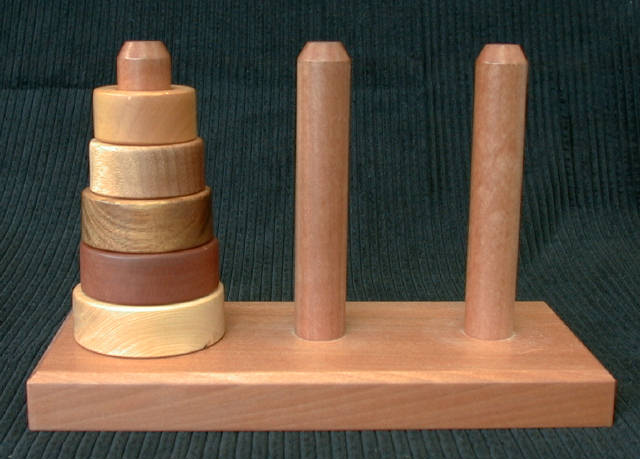
\includegraphics[width=0.89\textwidth]{images/hanoi}
	\end{figure}
\end{frame}

\begin{frame}{Towers of Hanoi}
	\begin{block}{Output - 3 blocks}
move from A to B.

move from A to C.

move from B to C.

move from A to B.

move from C to A.

move from C to B.

move from A to B.
	\end{block}
\end{frame}


\end{document}

